% Describe your system/solution design.
% Include figures with \begin{figure}...\end{figure} as needed.

\subsection{Top Level Architecture}
The top-level UVM architecture for the Shift Register is shown in Figure 1. Due to the simplicity of the DUT, a single-agent UVM environment was selected. The Shift Register contains only one interface and a small amount of control signals, therefore, only one Sequencer, Driver, and Monitor were required. A multi-agent architecture was considered unnecessary because it would increase development effort without improving verification functional coverage.

The Sequencer and Sequence generate abstract test scenarios known as transactions and forward them to the Driver. The implemented sequence executes approximately 100 randomized multidirectional bit-shifting tests with randomized values for shift enable, active-low reset, and serial input. Randomized constrained testing was chosen over purely directed testing because it increases scenario diversity, as well as improving the probability of detecting corner-case failures.

The Driver converts transaction-level stimulus into pin-level signal activity through the interface. The Interface provides connectivity between the Driver, Monitor, and DUT while simplifying signal management.

The Monitor passively observes DUT activity and captures both applied inputs and resulting outputs into transaction objects. These transactions are forwarded to the Scoreboard.

The Scoreboard serves as the primary checking component. It compares actual DUT outputs captured by the Monitor against expected outputs generated by the Predictor. The Predictor acts as a golden reference model and computes correct shift register behavior based on transaction inputs.

This modular UVM environment improves debuggability through structured reporting phases and improves scalability through reusable verification components. Although effective, UVM introduces substantial development overhead. For a DUT as simple as a Shift Register, a conventional SystemVerilog testbench could provide equivalent functional verification with lower implementation effort. However, UVM was selected to demonstrate industry-standard verification methodology and future scalability/reusability.
\begin{figure}[h]
    \centering
    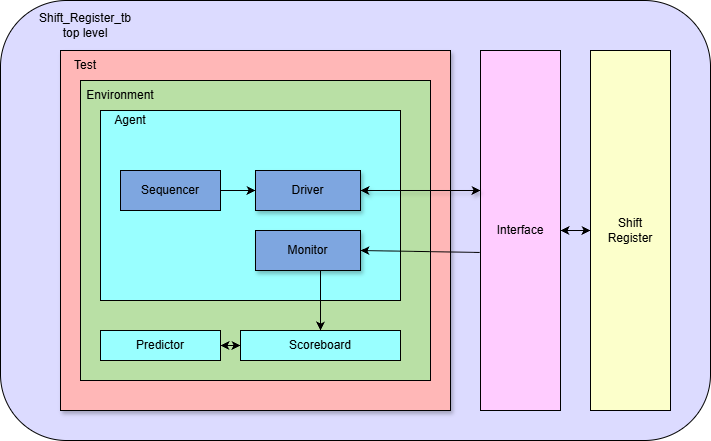
\includegraphics[width=1\linewidth]{figures/Shift_register_RTL.drawio.png}
    \caption{Shift Register Top Level Diagram}
    \label{fig:placeholder}
\end{figure}

\subsection{Deeper Dive into Code}
\subsubsection{Interface}

Figure 2 down below captures a snippet of the Shift Register IF. The Interface, as stated above, sends signals to and from the DUT to the testbench, using modports. All signals can be seen through each instantiation of the modport, DUT, being the signals inputted inside the DUT, while tester, being the I/O from the testbench.

\begin{figure}[h]
    \centering
    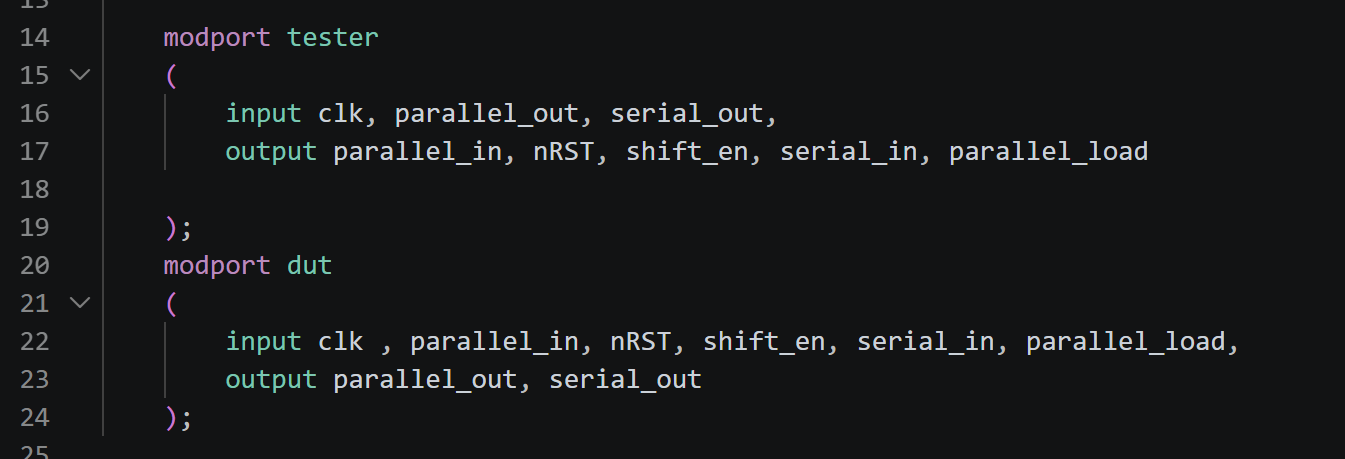
\includegraphics[width=1\linewidth]{figures/IF.png}
    \caption{Shift Register Interface modports}
    \label{fig:placeholder}
\end{figure}

\subsubsection{Driver}


Figure 3 below captures a snippet of the Driver. In the driver, the run phase is responsible for continuously receiving transactions from the sequencer. It then, pushes them to the DUT. 

Inside the forever loop, the driver calls \texttt{seq\_item\_port.get\_next\_item(req\_item)} to recieve the next randomized transaction. This transaction contains random values for \texttt{nRST}, \texttt{shift\_enable}, and \texttt{serial\_in}. The driver, then waits until the next negative edge of the clock, and drives these values into the virtual interface connected to the DUT. The reason we want to drive on the negative edge of the clock is because it allows inputs to stabilize before the DUT samples them on the following positive edge.

After the positive edge of the clock, the driver calls  \texttt{seq\_item\_port.item\_done()} to notify the sequencer that the transaction has completed, and the next item can be sent.

\begin{figure}[h]
    \centering
    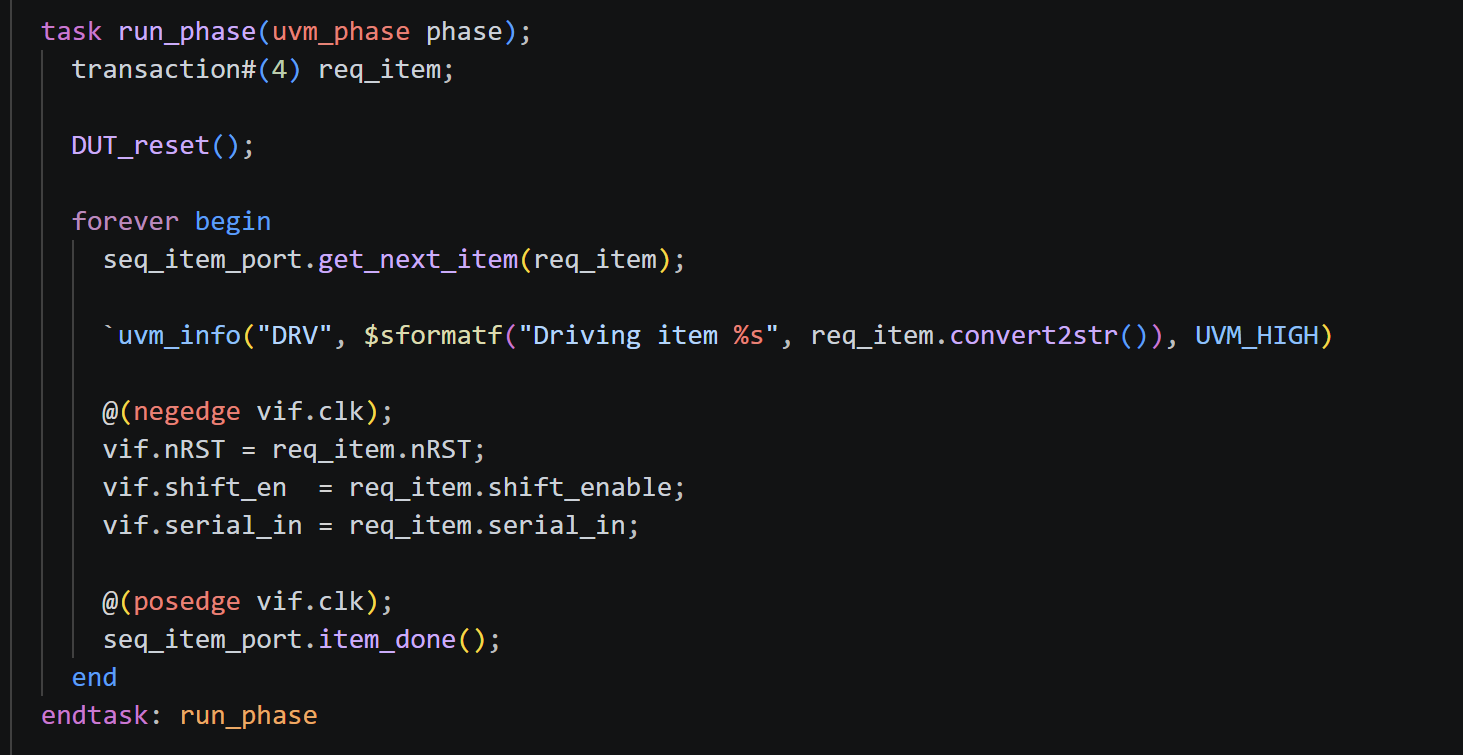
\includegraphics[width=1\linewidth]{figures/Driver.png}
    \caption{Shift Register Driver}
    \label{fig:placeholder}
\end{figure}


\subsubsection{Monitor}

Figure 4 captures a snippet of the Shift Register Monitor. The Monitor is responsible for passively observing the DUT interface and converting signal activity into transaction objects. Unlike the Driver, the Monitor does not control the DUT. Instead, it samples the interface signals and sends the observed information to other UVM components for checking and coverage collection.

In this design, the Monitor uses analysis ports to forward transactions. One stream captures the stimulus applied to the DUT, while the other captures the DUT output response. This separation allows the Predictor and Scoreboard to compare the expected and actual behavior of the Shift Register.

The Monitor samples signals around the clock edge so that the captured transaction reflects the DUT behavior after inputs have been applied and the output has had time to update. This is important because incorrect sampling timing can cause race conditions, where the Scoreboard compares an expected value against an output value from the wrong cycle.

The Monitor also supports functional coverage collection. By observing reset, shift enable, serial input, and output behavior, the Monitor helps measure whether the randomized sequence has exercised the important Shift Register scenarios.
\begin{figure}[h]
    \centering
    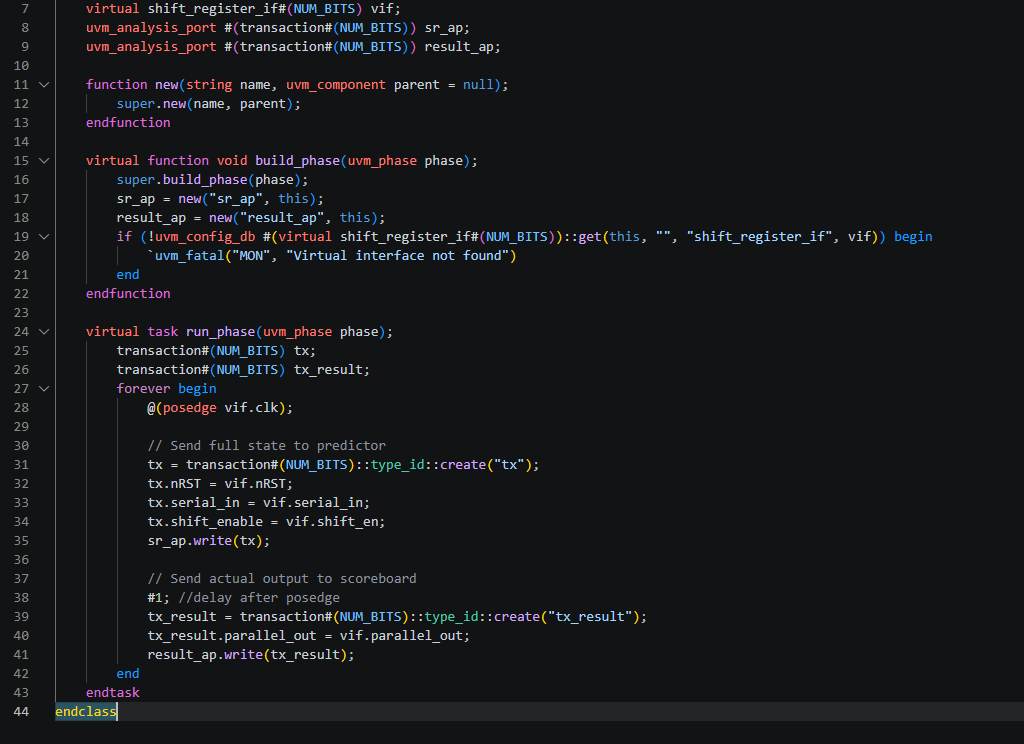
\includegraphics[width=1\linewidth]{figures/Monitor.png}
    \caption{Shift Register Monitor}
    \label{fig:placeholder}
\end{figure}

\subsubsection{Scoreboard}

Figures 5 and 6 below captures a snippet of the Scoreboard. The main function of the scoreboard is to compare expected output by the predictor, against actual output from DUT. 

In this design, the scoreboard uses two analysis implementation ports \texttt{exp\_imp} and \texttt{act\_imp}, to receive two separate streams of the transactions. 

The \texttt{exp\_imp} port receives the expected transaction from the predictor and stores it inside the queue named \texttt{exp\_q}. These queues are vital for the scoreboard because the expected and actual transactions might not come at the same time. The scoreboard then, stores them temporarily until both are available.

Once each queue contains a transaction item, the Scoreboard removes the oldest expected/actual transaction using \texttt{pop\_front()} and compares their \texttt{parallel\_out} values. If they match, the pass count is incremented, and the compare-pass message is printed. If values dont match, fail count is incremented, and UVM error is reported. 

Finally, during the \texttt{report\_phase}, the scoreboard prints the final number of passing and failing comparisons.

\begin{figure}[h]
    \centering
    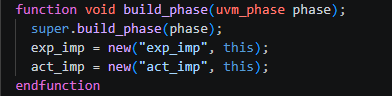
\includegraphics[width=1\linewidth]{figures/Scoreboard_imp.png}
    \caption{Shift Register Scoreboard imp}
    \label{fig:placeholder}
\end{figure}

\begin{figure}[h]
    \centering
    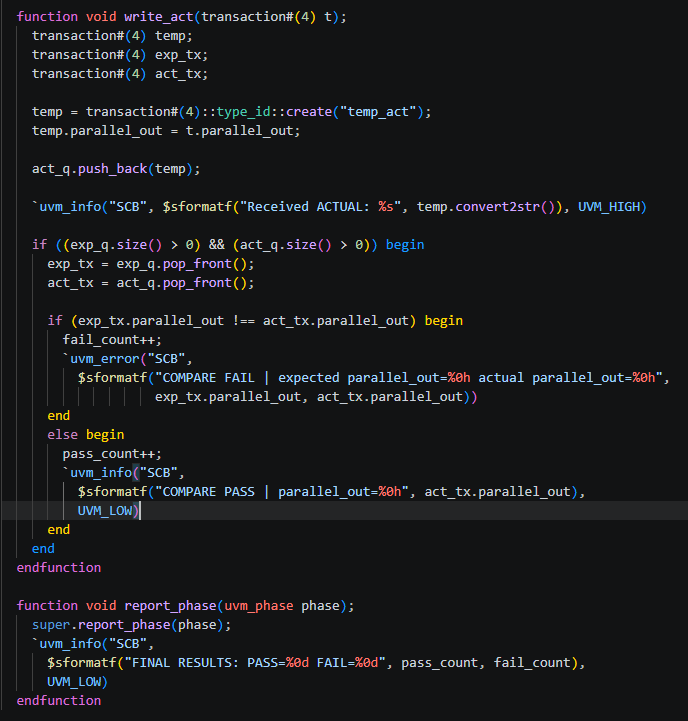
\includegraphics[width=1\linewidth]{figures/Scoreboard.png}
    \caption{Shift Register Scoreboard}
    \label{fig:placeholder}
\end{figure}

\subsubsection{Predictor}
Figure 7 Captures the essence of the Predictor. The predictor is responsible for generating the expected output of the shift register. 

In this design, the predictor extends \texttt{uvm\_subscriber}, which allows it to receive transactions thorough the \texttt{write()} function. The main variable used is \texttt{model\_q}, which represents the Predictor's golden reference model of the Shift Register. On every transaction, the Predictor updates that variable based on reset, as well as shift enable signals.

If \texttt{nRST} is low, the Predictor accurately models the DUT's reset behaviour by reseting the output to all ones. IF reset is not active and \texttt{shift\_enable} is high, the predictor shifts in \texttt{serial\_in}. The direction of shift depends on the \texttt{SHIFT\_MSB} parameter, and the size of \texttt{parallel\_out} depends on the \texttt{NUM\_BITS} parameter. After updating its internal golden reference model, the predictor assigns \texttt{model\_q} to \texttt{parallel\_out} and sends this expected transaction to the scoreboard through \texttt{predictor\_ap}

\begin{figure}[h]
    \centering
    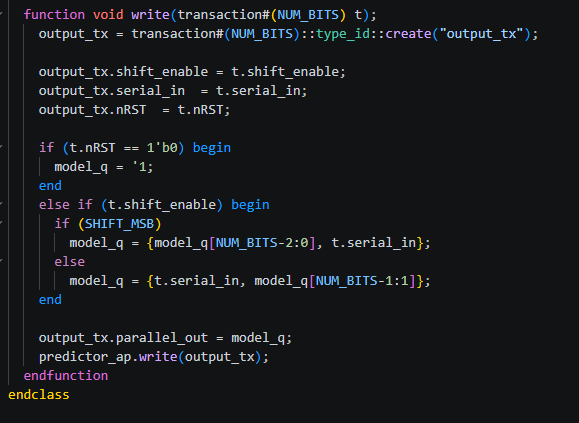
\includegraphics[width=1\linewidth]{figures/Predictor.png}
    \caption{Shift Register Predictor}
    \label{fig:placeholder}
\end{figure}

\subsubsection{Sequence}

Figure 8 captures a snippet of the Sequence. The Sequence is responsible for generating randomized transaction items that will be sent to the Driver through the Sequencer. In the \texttt{body()} task, a transaction object named \texttt{req\_item} is created repeatedly based on the value of \texttt{trans\_c}. Each transaction is started using \texttt{start\_item(req\_item)}, randomized using \texttt{req\_item.randomize()}, and then completed using \texttt{finish\_item(req\_item)}.

The randomization step generates different values for the transaction fields, such as \texttt{nRST}, \texttt{shift\_enable}, and \texttt{serial\_in}. If randomization fails, the sequence reports a fatal UVM error. This design allows the testbench to automatically create many randomized shift register scenarios, which improves coverage compared to manually writing each directed test.

\begin{figure}[h]
    \centering
    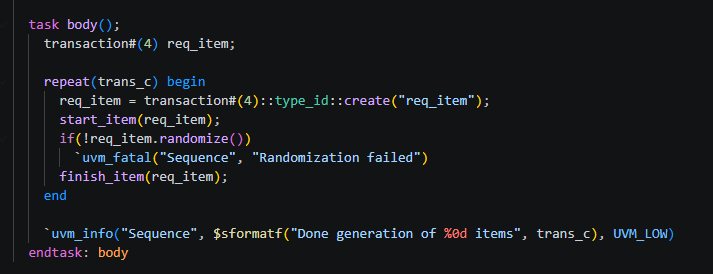
\includegraphics[width=1\linewidth]{figures/Sequence.png}
    \caption{Shift Register Sequence}
    \label{fig:placeholder}
\end{figure}